\documentclass[a4paper,10pt]{article}
\usepackage[utf8]{inputenc}
\usepackage{graphicx}
\usepackage{float}

\begin{document}

\section*{Trabalho de Programação para Dispositivos Móveis}

O trabalho consiste em criar uma estrutura que une pessoas com trocado a pessoas que precisam de troco. A data limite para entrega é até dia \textbf{10/06} e pode ser feito por \textbf{grupos de até 4 pessoas}.
Considerações:
\begin{itemize}
  \item O trabalho deve ser feito tendo como base o SDK 19 (Kit Kat);
  \item O dropdown UF deve ser preenchido com todas as UF's;
  \item Na tela \textbf{Tenho/Preciso de Troco} o valor que aparece para o usuário é o número de moedas/notas solicitadas;
  \item Na tela \textbf{Tenho/Preciso de Troco} após clicar em enviar deve aparecer um Toast informando o valor total solicitado e quantidade solicitada para cada nota/moeda; e
  \item O fluxo da aplicação deve ser \textbf{Tela Inicial} $>$ \textbf{Tela de Cadastro} $>$ \textbf{Tela de Tenho/Preciso de Troco} $>$ \textbf{Tela Inicial}.
\end{itemize}

As telas de cadastro e de troco \textbf{DEVEM SER VALIDADAS}:
\begin{itemize}
 \item Não deve ser permitido avançar sem preencher o cadastro todo; e
 \item Valores negativos para notas/moedas não são permitidos.
\end{itemize}

\newpage

\subsection*{Tela Inicial}

\begin{figure}[H]
    \centering
    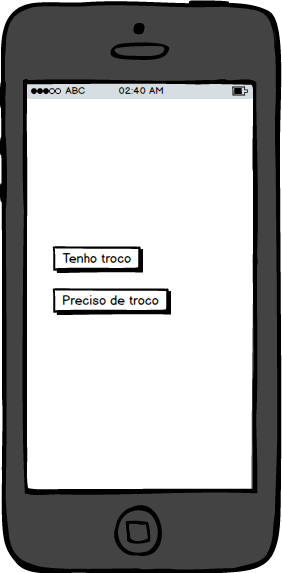
\includegraphics[scale=0.7]{t1_img/Inicial.png}
\end{figure}

\subsection*{Tela de Cadastro}

\begin{figure}[H]
    \centering
    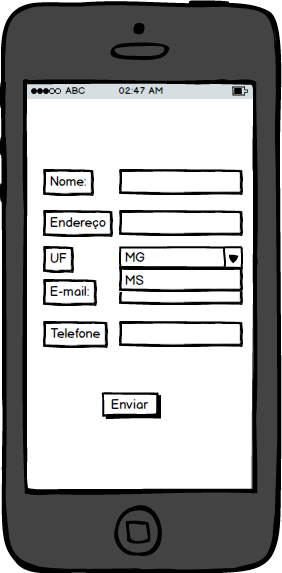
\includegraphics[scale=0.7]{t1_img/Cadastro.png}
\end{figure}

\subsection*{Tela Tenho/Preciso de Troco}

\begin{figure}[H]
    \centering
    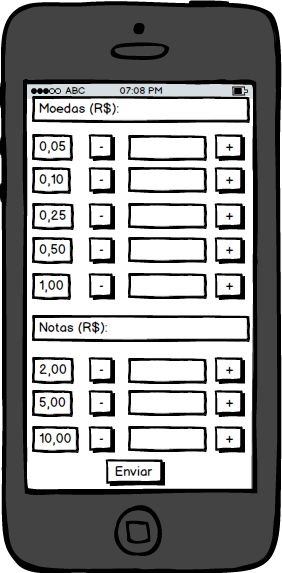
\includegraphics[scale=0.7]{t1_img/Troco.png}
\end{figure}

\end{document}
